\newcommand{\LRmath}[2]{\colorbox{lhsblue}{$#1$}\hspace{1mm}$\to$\hspace{1mm}\colorbox{rhsorange}{$#2$}}
% All diagrams are authored in LaTeX/TikZ. Native evidence is in examples/.
\definecolor{lhsblue}{HTML}{DCEBFA}
\definecolor{rhsorange}{HTML}{FFE5C7}
\definecolor{coarsepurple}{HTML}{7654A3}
\definecolor{smoothteal}{HTML}{267A68}
\tikzset{lhs/.style={box,fill=lhsblue,draw=blue!50!black},
 rhs/.style={box,fill=rhsorange,draw=orange!60!black},
 ext/.style={box,fill=black!5,draw=black!45},
 clayer/.style={draw=coarsepurple,very thick,rounded corners,inner sep=4mm},
 slayer/.style={draw=smoothteal,thick,dashed,rounded corners,inner sep=4mm},
 reuse/.style={arr,draw=smoothteal,thick},
 atom/.style={draw=black!50,rounded corners,fill=black!3,minimum height=7mm,font=\small},
 sat/.style={draw=smoothteal,double,rounded corners,inner sep=4mm}}
\newcommand{\MathLegend}{%
\begin{figure}[!htbp]\centering
\begin{tikzpicture}[node distance=8mm]
\node[lhs,text width=25mm] (l) {\textbf{LHS}\\matched facts};
\node[rhs,text width=25mm,right=of l] (r) {\textbf{RHS}\\constructed facts};
\node[ext,text width=25mm,right=of r] (e) {\textbf{External}\\input obligation};
\node[box,text width=25mm,right=of e,draw=smoothteal,double] {\textbf{Saturated}\\retained body};
\node[below=9mm of l,draw=coarsepurple,very thick,rounded corners,inner sep=3pt,font=\small] {Coarse layer $C$};
\node[below=9mm of e,draw=smoothteal,dashed,thick,rounded corners,inner sep=3pt,font=\small] {Smooth layer $S$};
\end{tikzpicture}
\caption{The v0.2.1 palette is retained. In rule diagrams blue/orange mark
matched/constructed facts, and purple/teal outlines mark coarse/smooth layers.
In native e-graph snapshots blue means present at entry and orange means added
since entry; purple/teal dashed clusters identify child/root e-classes, not layers.
Each caption specifies which kind of object and edge is being shown.}
\label{fig:legend}
\end{figure}}

\newcommand{\MathEgraph}{%
\begin{figure}[!htbp]\centering
\begin{minipage}[t]{.42\linewidth}\centering
\textbf{Before: $a+(b+c)$}\\[4pt]
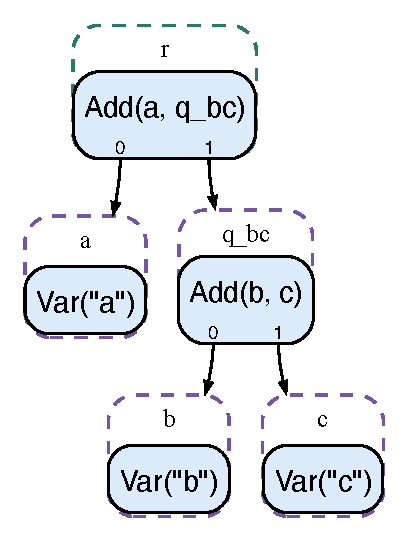
\includegraphics[width=\linewidth]{figures/native/entry.pdf}\\
\small 2 Add nodes; 5 Math e-classes
\end{minipage}\hfill
\begin{minipage}[t]{.55\linewidth}\centering
\textbf{After one associativity application}\\[4pt]
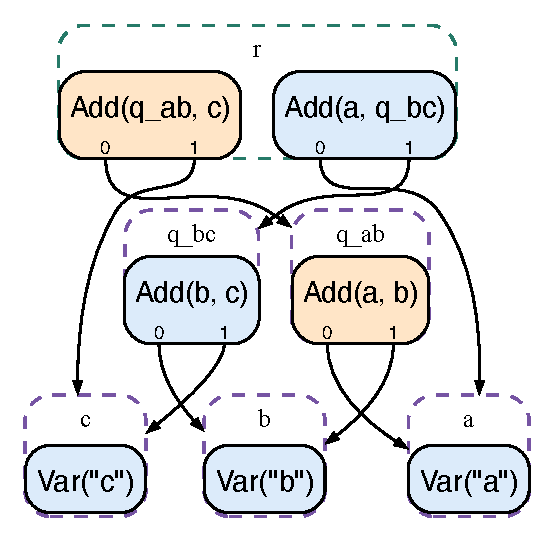
\includegraphics[width=\linewidth]{figures/native/assoc.pdf}\\
\small 4 Add nodes; 6 Math e-classes
\end{minipage}
\caption{Read the change from left to right. Native egglog introduces
Add$(a,b)$ and Add$(q_{ab},c)$ (orange) and unions the latter with the existing
root $r$. Blue nodes were already present. Dashed enclosures are native e-classes;
numbered ports are argument positions, and arrows terminate at child classes.
Both graphs come from executable prefixes of \texttt{math-mini-trace.egg}, through
egglog's own DOT exporter. Var's String payloads are inlined into its label.}
\label{fig:math-egraph}
\end{figure}}

\newcommand{\MathBinding}{%
\begin{figure}[!htbp]\centering
\begin{tikzpicture}[node distance=5mm and 20mm]
\node[rhs,text width=48mm] (v) {Associativity output port\\$v=\mathrm{Add}(a,b)$};
\node[ext,text width=48mm,below=of v] (c) {Carried port\\$c=\mathrm{Var}(\text{``c''})$};
\node[lhs,text width=43mm,right=of v] (x) {Commutation input\\$x\mapsto v$};
\node[lhs,text width=43mm,right=of c] (y) {Commutation input\\$y\mapsto c$};
\draw[reuse] (v)--node[above,font=\small]{$\rho(x)$}(x);
\draw[reuse] (c)--node[above,font=\small]{$\rho(y)$}(y);
\end{tikzpicture}
\caption{A concrete relative binding from the native Add trace: the next rule
matches Add$(v,c)$, so its formal variables become $x=v$ and $y=c$. This is a
port map, not addition of numeric binding offsets. The producer-to-consumer row
witness is recorded in the evidence file.}
\label{fig:math-binding}
\end{figure}}

\newcommand{\MathLayers}{%
\begin{figure}[!htbp]\centering
\begin{tikzpicture}
\node[lhs,text width=53mm] (l0) at (0,0) {\textbf{LHS}\quad $a+(b+c)$};
\node[rhs,text width=53mm] (r0) at (7,0) {\textbf{RHS}\quad $(a+b)+c$};
\draw[arr] (l0)--node[above,font=\small]{$R_{\rm assoc}$}(r0);
\node[lhs,text width=53mm] (l1) at (0,-3.1) {\textbf{LHS}\quad $v+c$};
\node[rhs,text width=53mm] (r1) at (7,-3.1) {\textbf{RHS}\quad $c+v$};
\draw[arr] (l1)--node[above,font=\small]{$R_{\rm comm}$}(r1);
\draw[reuse] (r0.south)--++(0,-8mm)-|node[pos=.25,above,font=\small]{$v=a+b$; same $c$}(l1.north);
\begin{scope}[on background layer]
\node[clayer,fit=(l0)(r0),label={[font=\small,text=coarsepurple]above:coarse rule layer $C_0$: one coarse rule composition}] {};
\node[slayer,fit=(l1)(r1),label={[font=\small,text=smoothteal]below:smooth rule layer $S_0$: one smooth rule composition}] {};
\end{scope}
\end{tikzpicture}
\caption{A concrete CS unit from \texttt{math.egg}. The first step requires the
external entry Add$(a,\mathrm{Add}(b,c))$; the second reads the associativity
output and needs no new external fact. The repeated orange/blue expression is
one reused node, shown in two occurrence roles, not duplicated storage. Labels
$C_0,S_0$ describe this selected interface, not globally unique runtime layer IDs.}
\label{fig:math-layers}
\end{figure}}

\newcommand{\MathGuard}{%
\begin{figure}[!htbp]\centering
\begin{tikzpicture}[node distance=8mm and 14mm]
\node[lhs,text width=35mm] (l) {\textbf{LHS}\quad $a/b$};
\node[rhs,text width=42mm,right=of l] (r) {\textbf{RHS}\quad $a\,b^{-1}$};
\node[ext,text width=60mm,below=of l,xshift=27mm] (g) {Required fact: \texttt{is-not-zero}$(b)$};
\draw[arr] (l)--node[above,font=\small]{$R_{\rm div}$}(r);
\draw[reuse] (g.north)--++(0,4mm);
\end{tikzpicture}
\caption{Why a binding is not enough. The guarded division rule is copied from
\texttt{math.egg}: a native check confirms that it does not apply without
\texttt{is-not-zero}$(b)$ and applies after that fact is supplied. This illustrates
an external obligation; it does not independently establish that the supplied
mathematical assertion is true.}
\label{fig:math-guard}
\end{figure}}

\newcommand{\MathCSCS}{%
\begin{figure}[!htbp]\centering
\begin{tikzpicture}[node distance=6mm and 8mm]
\node[coarse,text width=54mm] (c1) {$C_1$: Add associativity\\\LRmath{a+(b+c)}{v+c}};
\node[smooth,text width=54mm,right=of c1] (s1) {$S_1$: Add commutation\\\LRmath{v+c}{c+v}};
\node[ext,text width=96mm,below=of c1,xshift=31mm] (i) {New outer context: $p\,r$, with $r=[c+v]$\\carry the fact $v=[a+b]$ from $\CS_1$};
\node[coarse,text width=54mm,below=of i,xshift=-31mm] (c2) {$C_2$: distribution layer\\\LRmath{p(c+v)}{pc+pv}};
\node[smooth,text width=54mm,right=of c2] (s2) {$S_2$: distribution inside $pv$\\\LRmath{p(a+b)}{pa+pb}};
\draw[arr] (c1)--(s1);\draw[reuse] (s1.south)|-(i.east);
\draw[arr] (i)--(c2);\draw[arr] (c2)--(s2);
\end{tikzpicture}
\caption{A native-checked CSCS example using associativity, commutation, and
distribution from \texttt{math.egg}. Distribution may match several retained
representatives; one is shown. The declared interface of $\CS_2$ carries the
Add$(a,b)$ fact, so its inner distribution step does not fetch it for free.
The fresh outer multiplication context is supplied only after $\CS_1$.}
\label{fig:math-cscs}
\end{figure}}

\newcommand{\MathCCSS}{%
\begin{figure}[!htbp]\centering
\begin{tikzpicture}[node distance=6mm and 10mm]
\node[coarse,text width=48mm] (ca) {$C_A$\\\LRmath{a+(b+c)}{(a+b)+c}};
\node[coarse,text width=48mm,right=of ca] (cm) {$C_M$\\\LRmath{a(bc)}{(ab)c}};
\node[smooth,text width=48mm,below=10mm of ca] (sa) {$S_A$\\\LRmath{(a+b)+c}{c+(a+b)}};
\node[smooth,text width=48mm,right=of sa] (sm) {$S_M$\\\LRmath{(ab)c}{c(ab)}};
\draw[arr] (ca)--(sa);\draw[arr] (cm)--(sm);
\draw[reuse,<->] (ca)--node[above,font=\scriptsize]{shared $a,b,c$}(cm);
\begin{scope}[on background layer]
\node[clayer,fit=(ca)(cm),label={[font=\small]above:merged coarse layer $C_A\cup C_M$}] {};
\node[slayer,fit=(sa)(sm),label={[font=\small]below:merged smooth layer $S_A\cup S_M$}] {};
\end{scope}
\end{tikzpicture}
\caption{CCSS with real Add/Mul rules from \texttt{math.egg}. Both input trees
are declared initially and share $a,b,c$; there is no S-to-C dependency.
The restricted native fragment saturates to 12 Add and 12 Mul rows. Layer
outlines indicate regrouping, not deletion of the four original compositions.}
\label{fig:math-ccss}
\end{figure}}

\newcommand{\MathSaturated}{%
\begin{figure}[!htbp]\centering
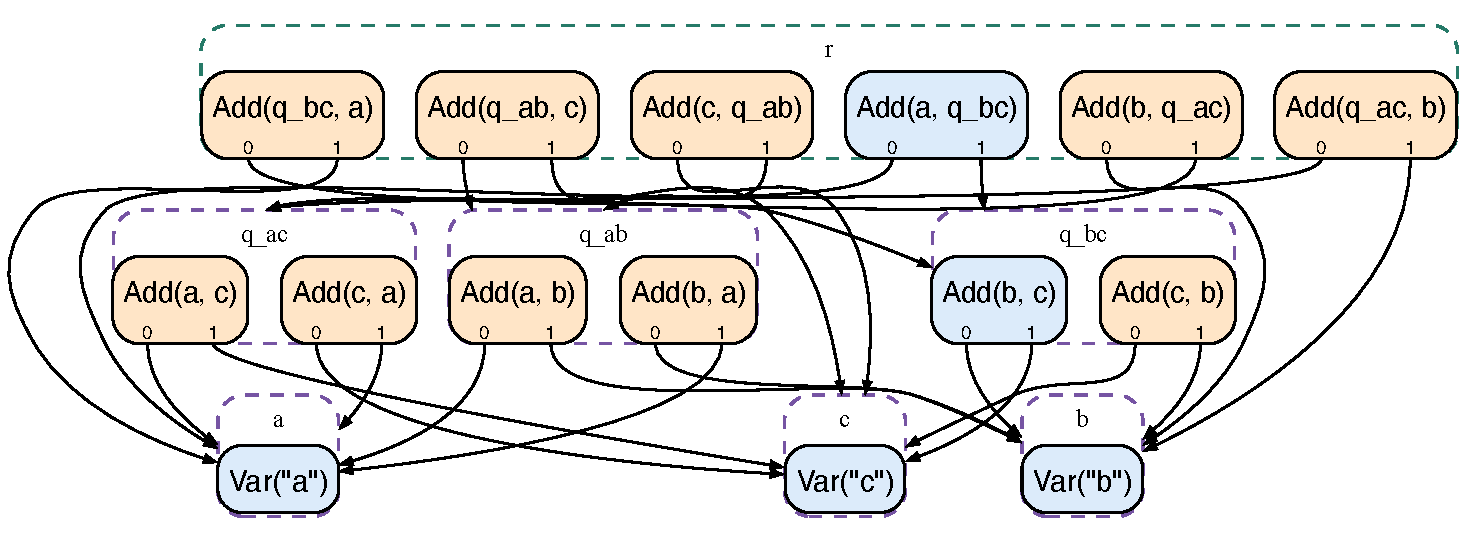
\includegraphics[width=\linewidth]{figures/native/saturated.pdf}
\caption{The Add body exported by the mini \texttt{math.egg} fragment. This
figure is generated from egglog's own \texttt{--to-dot} serializer: dashed
clusters are e-classes, solid boxes are e-nodes, and numbered ports preserve
ordered child positions. The paper-side transformation only inlines Var string
payloads and annotates the entry-relative colours; it checks that every Math
node and ordered child edge from the native DOT survives. The graph has 12 Add
nodes, three Var nodes, and seven Math e-classes.}
\label{fig:math-saturated}
\end{figure}}

\newcommand{\MathVisibility}{%
\begin{figure}[!htbp]\centering
\begin{tikzpicture}[node distance=7mm and 9mm]
\node[lhs,text width=33mm] (add) {\textbf{LHS}\\Add$(1,2)$};
\node[rhs,text width=33mm,right=of add] (three) {\textbf{RHS}\\Const$(3)$};
\node[ext,text width=43mm,right=of three] (hidden) {Add$(1,2)$ retained\\\textbf{subsumed / hidden}};
\draw[arr] (add)--node[above,font=\scriptsize]{fold + union}(three);
\draw[arr] (three)--node[above,font=\scriptsize]{prune}(hidden);
\node[below=8mm of three,font=\small] {Same retained equality does not imply the same matching visibility.};
\end{tikzpicture}
\caption{The constant-fold and prune rules of \texttt{math.egg}. Native execution
retains the Add row after subsumption but marks it hidden. An exported local state must
record this flag; an instance lease depending on its visibility needs rechecking.}
\label{fig:math-visibility}
\end{figure}}

\newcommand{\MathFractalBinding}{%
\begin{figure}[!htbp]\centering
\begin{tikzpicture}[node distance=7mm and 13mm]
\node[lhs,text width=43mm] (before) {Current binding\\$(u_k,v_k,x)$};
\node[rhs,text width=68mm,right=of before] (after) {Next residual binding\\$(D_xu_k,\ \int v_k\,dx,\ x)$};
\draw[reuse] (before)--node[above,font=\small]{$\rho_{\rm IBP}$}(after);
\node[below=5mm of after,font=\small] {Construct, construct, carry: same transfer at every depth.};
\end{tikzpicture}
\caption{The binding transfer of the integration-by-parts rule in \texttt{math.egg}.
Growing expression depth does not require a new transfer template: the same
Diff/Integral constructors and carried integration variable define each step.}
\label{fig:math-fractal-binding}
\end{figure}}

\newcommand{\MathTrigger}{%
\begin{figure}[!htbp]\centering
\begin{tikzpicture}[node distance=7mm]
\node[ext,text width=31mm] (i) {External entry\\$I_0=\int u_0v_0\,dx$};
\node[coarse,text width=34mm,right=of i] (c) {Coarse IBP\\creates $u_1,v_1,I_1$};
\node[smooth,text width=42mm,right=of c] (s) {Smooth recursive tail\\$I_1\to I_2\to\cdots$};
\draw[arr] (i)--(c);\draw[reuse] (c)--(s);
\end{tikzpicture}
\caption{A one-step trigger for the selected IBP family. The first application
acquires an external entry; subsequent residual applications reuse constructed
facts. Other families can have longer, nonuniform effect-producing prefixes.}
\label{fig:math-trigger}
\end{figure}}

\newcommand{\MathDissipative}{%
\begin{figure}[!htbp]\centering
\begin{tikzpicture}[node distance=7mm]
\node[lhs,text width=28mm] (a) {$1+1+1+1+1$\\four pending adds};
\node[rhs,text width=24mm,right=of a] (b) {$2+1+1+1$\\$\mu=3$};
\node[rhs,text width=24mm,right=of b] (c) {$3+1+1$\\$\mu=2$};
\node[rhs,text width=24mm,right=of c] (d) {$\cdots\to5$\\$\mu=0$};
\draw[arr] (a)--(b);\draw[arr] (b)--(c);\draw[arr] (c)--(d);
\node[ext,text width=110mm,below=8mm of b,xshift=16mm] {One Const$(1)$ e-node can serve all five positions.\\Native run: four Add rows remain; Const rows grow from one to five.};
\end{tikzpicture}
\caption{A dissipative composition using the native constant-fold rule from
\texttt{math.egg}. The initial expression is left-associated; outer Add facts
are part of the declared entry. The remaining work frontier decreases, not the
stored fact set. No pruning is enabled in this example.}
\label{fig:math-dissipative}
\end{figure}}

\newcommand{\MathInfi}{%
\begin{figure}[!htbp]\centering
\begin{tikzpicture}[node distance=7mm]
\node[lhs,text width=115mm] (l) {\textbf{LHS}\quad $I_k=\int u_kv_k\,dx$};
\node[rhs,text width=115mm,below=of l] (r) {\textbf{RHS}\quad $u_kv_{k+1}-\boxed{I_{k+1}}$\\$u_{k+1}=D_xu_k,\quad v_{k+1}=\int v_k\,dx$};
\draw[arr] (l)--node[right,font=\small]{$R_{\rm IBP}$}(r);
\node[box,text width=115mm,below=of r,draw=smoothteal,dashed] (chain) {$I_0\ \to\ I_1\ \to\ I_2\ \to\ I_3\ \to\cdots$\\
$u_0,v_0$\quad $D_xu_0,\int v_0$\quad $D_x^2u_0,\int^2v_0$\quad $\cdots$};
\draw[reuse] (r)--(chain);
\end{tikzpicture}
\caption{A productive infi rule composition from the actual IBP rule. In the
\emph{IBP-only} fragment, the boxed residual regenerates the same pattern with
strictly deeper Diff/Integral arguments. Four native steps yield 11, 17, 23,
and 29 Math e-nodes. The all-depth argument requires the restricted theory;
full \texttt{math.egg} may simplify the derivative and terminate this family.}
\label{fig:math-infi}
\end{figure}}

\newcommand{\MathSummary}{%
\begin{figure}[!htbp]\centering
\begin{tikzpicture}[node distance=8mm and 14mm]
\node[lhs,text width=47mm] (full) {Repeated IBP effects\\$I_0\to I_1\to\cdots\to I_k$};
\node[rhs,text width=62mm,right=of full] (summary) {Endpoint summary\\$\displaystyle\sum_{j=0}^{k-1}(-1)^j u_jv_{j+1}+(-1)^k I_k$};
\node[ext,text width=103mm,below=of summary,xshift=-32mm] (query) {Required intermediate query: retrieve $I_j$ for $0\le j\le k$.\\Endpoint-only reduction does not answer every rule match.};
\draw[proposed] (full)--node[above,font=\scriptsize]{contract + Reduce}(summary);
\draw[proposed] (summary)--(query);
\end{tikzpicture}
\caption{How an infi composition could feed ripen: summarize the alternating
endpoint, but retain an indexed residual interface. This is a proposed contract
for the worked IBP family with additional exact additive laws, not a claim that the current Reduce DSL automatically
discovers or executes this alternating-sum summary.}
\label{fig:math-summary}
\end{figure}}

% The main reader-facing comparison: show the concrete object before naming the
% abstraction.  Two triggers remain distinct, while only the exported local
% state is grouped by exact comparison; this is cataloguing, not tier0 reuse.
\newcommand{\MathSharingComparison}{%
\begin{figure}[!htbp]\centering
\begin{tikzpicture}[node distance=10mm and 22mm]
\node[lhs,text width=49mm] (ra) {$T_R$: $a+(b+c)$\\own entry and obligations};
\node[rhs,text width=49mm,right=of ra] (la) {$T_L$: $(a+b)+c$\\own entry and obligations};
\node[box,text width=49mm,below=of ra] (rk) {$K_R$ after native ripen\\12 Add + 3 Var; 7 Math classes};
\node[box,text width=49mm,below=of la] (lk) {$K_L$ after native ripen\\12 Add + 3 Var; 7 Math classes};
\draw[arr] (ra)--(rk);\draw[arr] (la)--(lk);
\node[box,draw=smoothteal,double,text width=90mm,below=13mm of rk,xshift=37mm] (k)
 {Exact typed comparison: $K_R\cong K_L$\\Catalog: one body $K$; two separate trigger records\\$T_R\mapsto K$ and $T_L\mapsto K$, each with its value map};
\draw[reuse] (rk)--(k.north west);\draw[reuse] (lk)--(k.north east);
\end{tikzpicture}
\caption{Two different entries can produce the same body. These are catalog and
execution records, not e-class boxes. Native replays and exact comparison are
checked by the \texttt{math\_parenthesizations} regression. Equal counts alone
are insufficient: the comparison preserves all rows, ports and visibility.
The two entries remain distinct, and the live tier0 graph is not replaced.}
\label{fig:sharing-comparison}
\end{figure}}

\newcommand{\MathRecursiveArrays}{%
\begin{figure}[t]\centering
\begin{minipage}[t]{.48\linewidth}\centering
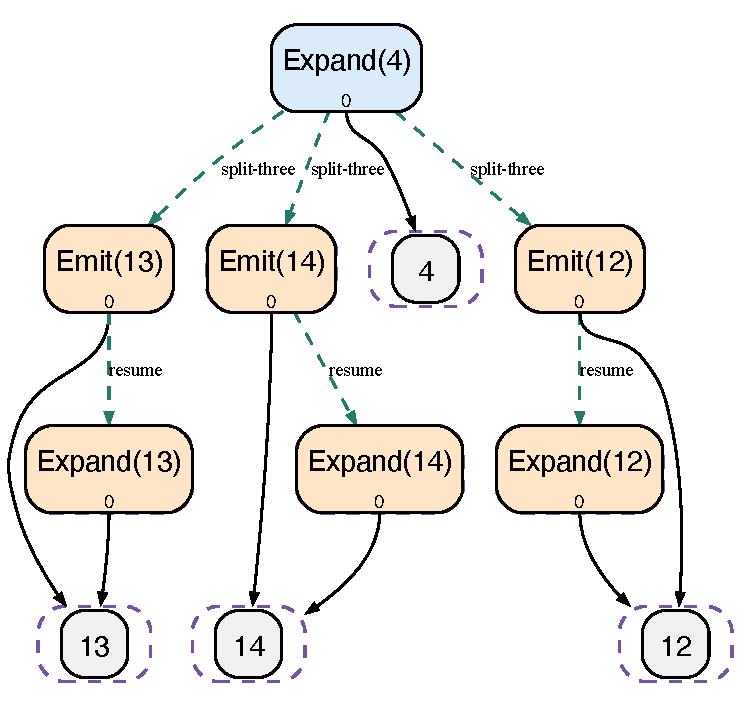
\includegraphics[width=\linewidth]{figures/native/recursive-tree.pdf}\\[-2pt]
\small Native recursive e-graph: \texttt{Expand(4)} produces
\texttt{Emit(12)}, \texttt{Emit(13)}, \texttt{Emit(14)}.
\end{minipage}\hfill
\begin{minipage}[t]{.48\linewidth}\centering
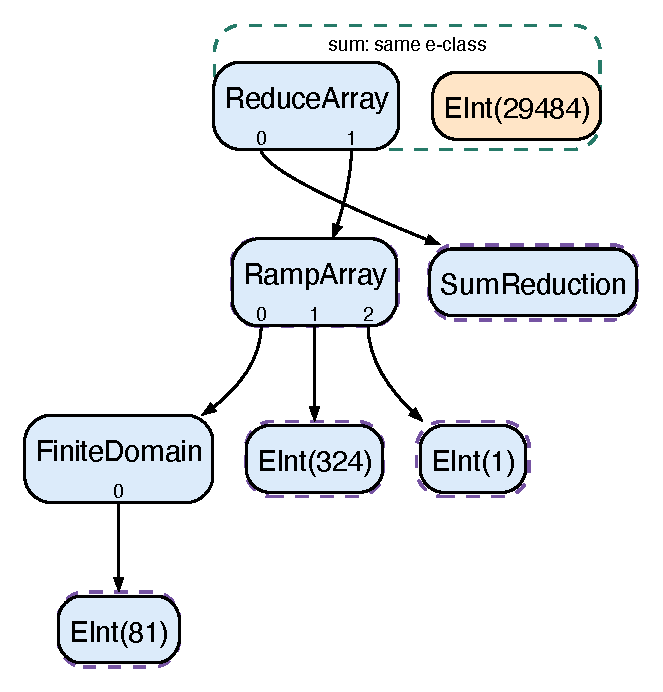
\includegraphics[width=\linewidth]{figures/native/recursive-array.pdf}\\[-2pt]
\small Native array-query graph after Bake: \texttt{RampArray(81,324,1)}
and \texttt{ReduceArray}.
\end{minipage}
\caption{The recursive-array case in two stages. The left graph is an executable
Math e-graph snapshot; solid edges are native child references and dashed
\texttt{split-three}/\texttt{resume} edges are explicitly labelled rule-instance
annotations. The right graph is the native tier2 array query produced from the
certified Bake law. Its paper annotation removes helper arithmetic alternatives,
but the remaining nodes and solid child-class edges are checked against the
native DOT export.}
\label{fig:recursive-array-graphs}
\end{figure}}
